\chapter{Operating System Support}
In the present section, we will examine the relationship between the middleware layer and the operating system (OS) layer. The task of any operating system is \textbf{to provide problem-oriented abstractions of the underlying physical resources}, it takes over the physical resources on a single node and manages them to present these resource abstractions through the system-call interface.


\section{Operating System Layer}
Users will only be satisfied if their middleware-OS combination has good performance. \textbf{Middleware runs on a variety of OS-hardware combinations.}  The OS running at a node provides its own flavour of abstractions of local hardware resources for processing, storage and communication.

The following image shows how the operating system layer at each of two nodes supports a \textbf{common middleware} layer in providing a distributed infrastructure for applications and services.

\begin{figure}[!h]
    \centering
    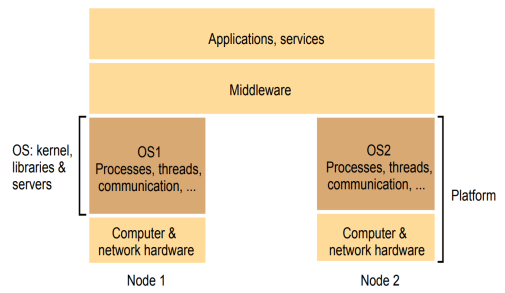
\includegraphics[width=.7\linewidth]{images/OperatingSystemSupport/operatingsystemlayer.png}
    \caption{Operating System Layer}
\end{figure}

The below image instead shows the \textbf{core OS functionality} that we shall be concerned with: process and thread management, memory management and communication between processes on the same computer.

\begin{figure}[!h]
    \centering
    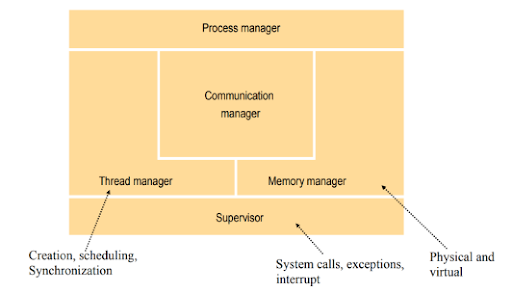
\includegraphics[width=.7\linewidth]{images/OperatingSystemSupport/osfunctionality.png}
    \caption{Core OS Functionality}
\end{figure}

The core OS components and their responsibilities are:
\begin{itemize}
    \item \textbf{Process manager:} creation of operations upon processes. A process is a unit of resource management, including an address space and one or more threads.
    \item \textbf{Thread manager:} thread creation, synchronisation and scheduling. Threads are scheduled activities attached to processes.
    \item \textbf{Communication manager:} communication between threads attached to different processes on the same computer.
    \item \textbf{Memory manager:} management of physical and virtual memory
    \item \textbf{Supervisor:} dispatching of interrupts, system call traps and other exceptions, control of memory management unit and hardware caches
\end{itemize}

\section{Process and Threads}
\begin{itemize}
    \item A \textbf{preocess} consists of an execution enviroment together with one or more \textbf{threads}
    \item A \textbf{thread} is the operating system abstraction of an activity
    \item An \textbf{execution environment} is the unit of resource management: a collection of local kernel-managed resources to which its threads have access. An execution environment primarily consists of:
        \begin{itemize}
            \item An \textbf{address space}
            \item \textbf{Thread synchronization and communication resources} such as semaphores and communication interfaces (sockets).
            \item \textbf{Higher-level resources} such as open files and windows
        \end{itemize}
\end{itemize}
Execution \textbf{environments} are normally \textbf{expensive} to create and manage, but \textbf{several threads can share them.}

Threads can be created and destroyed dynamically and the goal of having multiple threads of execution is to \textbf{maximise the degree of concurrent execution between operations}, thus enabling the overlap of computation with input and output, and enabling concurrent processing on multiprocessors.

\subsection{Address Space}
An address space is a unit of management of a process’s virtual memory. It is large and consists of one or more regions, separated by \textbf{inaccessible areas of virtual memory.}

\begin{figure}[!h]
    \centering
    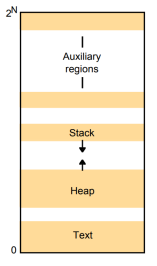
\includegraphics[width=.2\linewidth]{images/OperatingSystemSupport/addressSpace.png}
    \caption{Address Space}
\end{figure}

Each region is specified by the following properties:
\begin{itemize}
    \item Its dimension: lowest virtual address and size
    \item Permissions for the process’s threads: read/write/execute
    \item Direction of  grown: upwards or downwards
\end{itemize}
A \textbf{shared memory region} is one that is backed by the same physical memory as one or more regions belonging to other address spaces.
Processes therefore access identical memory contents in the regions that are shared, while their non-shared regions remain protected.
The uses of shared regions include the following:
\begin{itemize}
    \item \textbf{Libraries:} library code can be very large and would waste considerable memory if it was loaded separately into every process that used it
    \item \textbf{Kernel:} often the kernel code and data are mapped into every address space at the same location
    \item \textbf{Data sharing and communication:} two processes, or a process and the kernel, might need to share data in order to cooperate on some task
\end{itemize}

\subsection{Creation of a New Process}
For a distributed system, the design of the process-creation mechanism has to take into account the \textbf{utilisation of multiple computers}, consequently, the process-support infrastructure is divided into separate system services.
The creation of a new process can be separated into two independent aspects:
\begin{itemize}
    \item The \textbf{choice of a target host}, for example, the host may be chosen from among the nodes in a cluster of computers acting as a compute server. The choice of the node at which the new process will reside is a matter of policy:
        \begin{itemize}
            \item The transfer policy determines whether to situate a new process locally or remotely
            \item The location policy determines which node should host a new process selected for transfer
            \item Process location policies may be static or adaptive
        \end{itemize}
    \item The \textbf{creation of an execution environment:} once the host computer has been selected, a new process requires an execution environment consisting of an address space with initialised contents. There are \textbf{two approaches:}
        \begin{enumerate}
            \item The first is used where the address space is of a statically defined format. In this case, the address space regions are created from a list specifying their extent
            \item In the second approach, the address space can be defined with respect to an existing execution environment
        \end{enumerate}
\end{itemize}

\begin{figure}[!h]
    \centering
    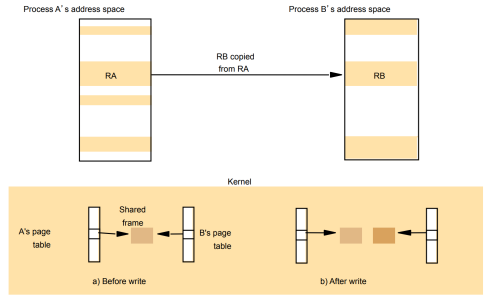
\includegraphics[width=.7\linewidth]{images/OperatingSystemSupport/executionenviroment.png}
    \caption{Creation of an Execution Environment}
\end{figure}

\subsection{Threads}
Advantages of enabling client and server processes to \textbf{possess more than one thread}.  They allow concurrency with I/O operation and computation in multiprocessor systems. Possible \textbf{advantages} of the multi-thread are:
\begin{itemize}
    \item Less expensive for creation and management
    \item Simpler to make resource sharing
\end{itemize}
Possible problems can be, instead, the mechanisms for concurrent programming.

\begin{figure}[!h]
    \centering
    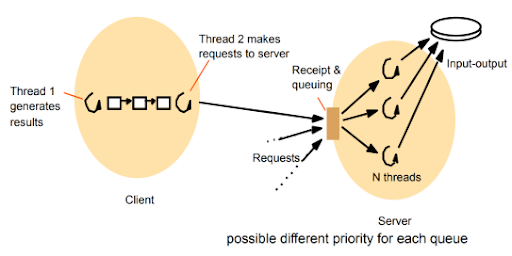
\includegraphics[width=.7\linewidth]{images/OperatingSystemSupport/threads.png}
    \caption{Thread Architecture}
\end{figure}

The previous image shows one of the possible \textbf{threading architectures}, the \textbf{worked pool architecture}. In its simplest form, the server creates a fixed pool of "worker" threads to process the requests when it starts up. The module marked "receipt and queuing" is typically implemented by an "I/O" thread, which receives requests from a collection of sockets or ports and places them on a shared request queue for retrieval by the workers. We may handle varying request priorities by introducing multiple queues into the worker pool architecture, so that the worker threads scan the queues in the order of decreasing priority.

Disadvantages:
\begin{itemize}
    \item Its \textbf{inflexibility}, the number of worker threads in the pool may be too few to deal adequately with the current rate of request arrival
    \item High level of switching between the I/O and worker threads as they manipulate the shared queue
\end{itemize}

Other types of architectures are:
\begin{itemize}
    \item \textbf{Thread-per-request architecture:} the I/O thread spawns a new worker thread for each request, and that worker destroys itself when it has processed the request against its designated remote object. This architecture has the advantage that the threads do not contend for a shared queue, and throughput is potentially maximized because the I/O thread can create as many workers as there are outstanding requests. Its disadvantage is the overhead of the thread creation and destruction operations.
    \item \textbf{Thread-per-connection architecture:} associates a thread with each connection. The server creates a new worker thread when a client makes a connection and destroys the thread when the client closes the connection.
    \item \textbf{thread-per-object architecture:} associates a thread with each remote object. An I/O thread receives requests and queues them for the workers, but this time there is a per-object queue.
\end{itemize}
The representation of these different architectures can be seen in the following image

\begin{figure}[!h]
    \centering
    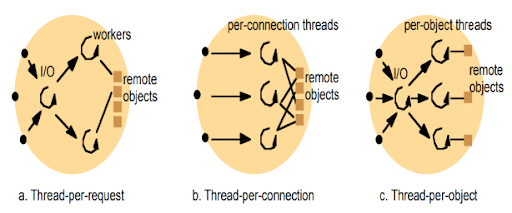
\includegraphics[width=.7\linewidth]{images/OperatingSystemSupport/typeofthread.png}
    \caption{Types of Thread Architecture}
\end{figure}
\newpage
The JAVA thread’s life cycle can be seen in the below image

\begin{figure}[!h]
    \centering
    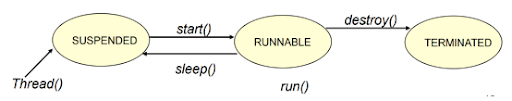
\includegraphics[width=.7\linewidth]{images/OperatingSystemSupport/javalifeciclethread.png}
    \caption{Java Thread's Lifecycle}
\end{figure}


\section{Scheduler and Thread}
Many kernels provide native support for multi-threaded processes, including Windows, Linux, Solaris, Mach and Mac OS X. These kernels provide thread-creation and management system calls, and they schedule individual threads. Some other kernels have only a single-threaded process abstraction. Multi-threaded processes must then be implemented in a library of procedures linked to application programs. We can say that threads are implemented at \textbf{application level}. In such cases, the kernel has no knowledge of these user-level threads and therefore cannot schedule them independently
Using thread at application level we have some advantages like:
\begin{itemize}
    \item Less cost to context change
    \item Possible to implement scheduling ad hoc
    \item Possible to create and manage larger number of possible threads
\end{itemize}
The \textbf{drawbacks} are:
\begin{itemize}
    \item Kernel cannot make thread scheduling
    \item Kernel cannot compare priorities of thread in different processes
    \item Thread cannot use multiprocessor concurrency
    \item A thread error blocks the process and all its threads
\end{itemize}
It is possible to \textbf{combine} the \textbf{advantages of user-level} and \textbf{kernel-level} threads implementations. Possible approaches:
\begin{itemize}
    \item Enable user-level code to provide scheduling hints to the kernel’s thread scheduler it is called \textbf{hybrid solution}
    \item Form of \textbf{hierarchical scheduling}
\end{itemize}


\section{Communication: invocation and call}
Communication is part of invocation and it can be implemented using different approches like:
\begin{enumerate}
    \item RPC
    \item RMI
    \item Message Passing
    \item Event Notification 
    \item System call
    \item Group Notification
\end{enumerate}
An important aspect of communication is the \textbf{performance provided by the mechanism used}. Fundamental aspects that can affect the performance are:
\begin{enumerate}
    \item \textbf{Type of communication} that can be \textit{synchronous} or \textbf{asynchronous}
    \item \textbf{Address space to cross}, it can be \textit{local} or \textit{remote}
    \item \textbf{Scheduling thread} that affect context change 
\end{enumerate}

\begin{figure}[!h]
    \centering
    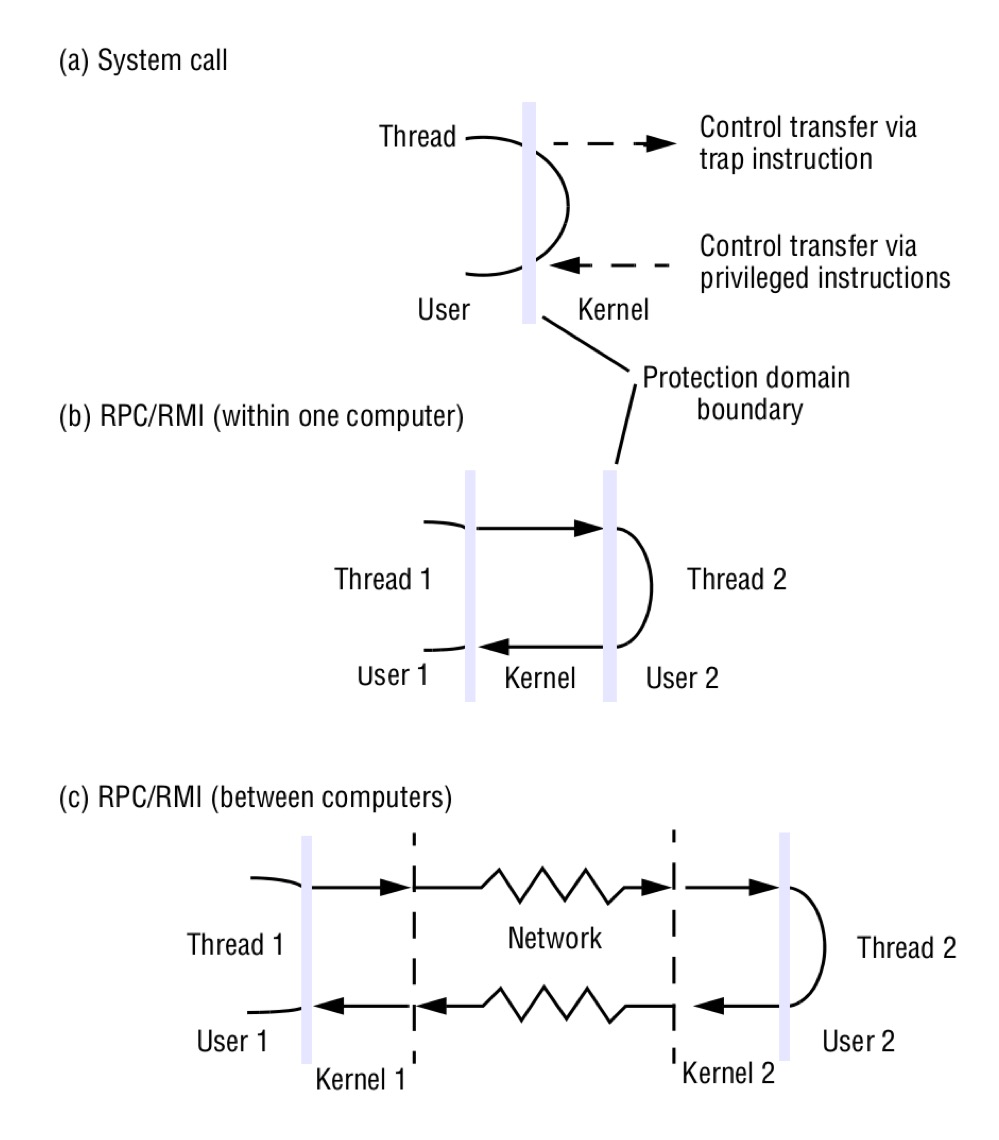
\includegraphics[width=.5\linewidth]{images/OperatingSystemSupport/topologyOfAddressSpace.jpeg}
    \caption{Topology of Address Space}
\end{figure}

\subsection{Lightweight Remote Procedure Call}
The previous image suggest that a \textit{cross-address-space} invocation is implemented within a computer exactly as it is between computers. Indeed Bershad developed a more efficient invocation mechanism for the case of two processes on the same machine called \textbf{lightweight RPC, LRPC}.

The LRPC design is based on optimization concerning \textbf{data copying} and \textbf{thread scheduling}. Instead of RPC parameters being copied between the kernel and user address spaces involved, the client and server are able to \textbf{pass arguments} and \textbf{return values} directly via an A stack.  The same stack is used by the client and server stubs. In LRPP, the \textbf{arguments are copied once:} when they are marshalled onto the A stack. There my be several A stacks in a shared region, because several threads in the same client may call the server at the same time.

\begin{figure}[!h]
    \centering
    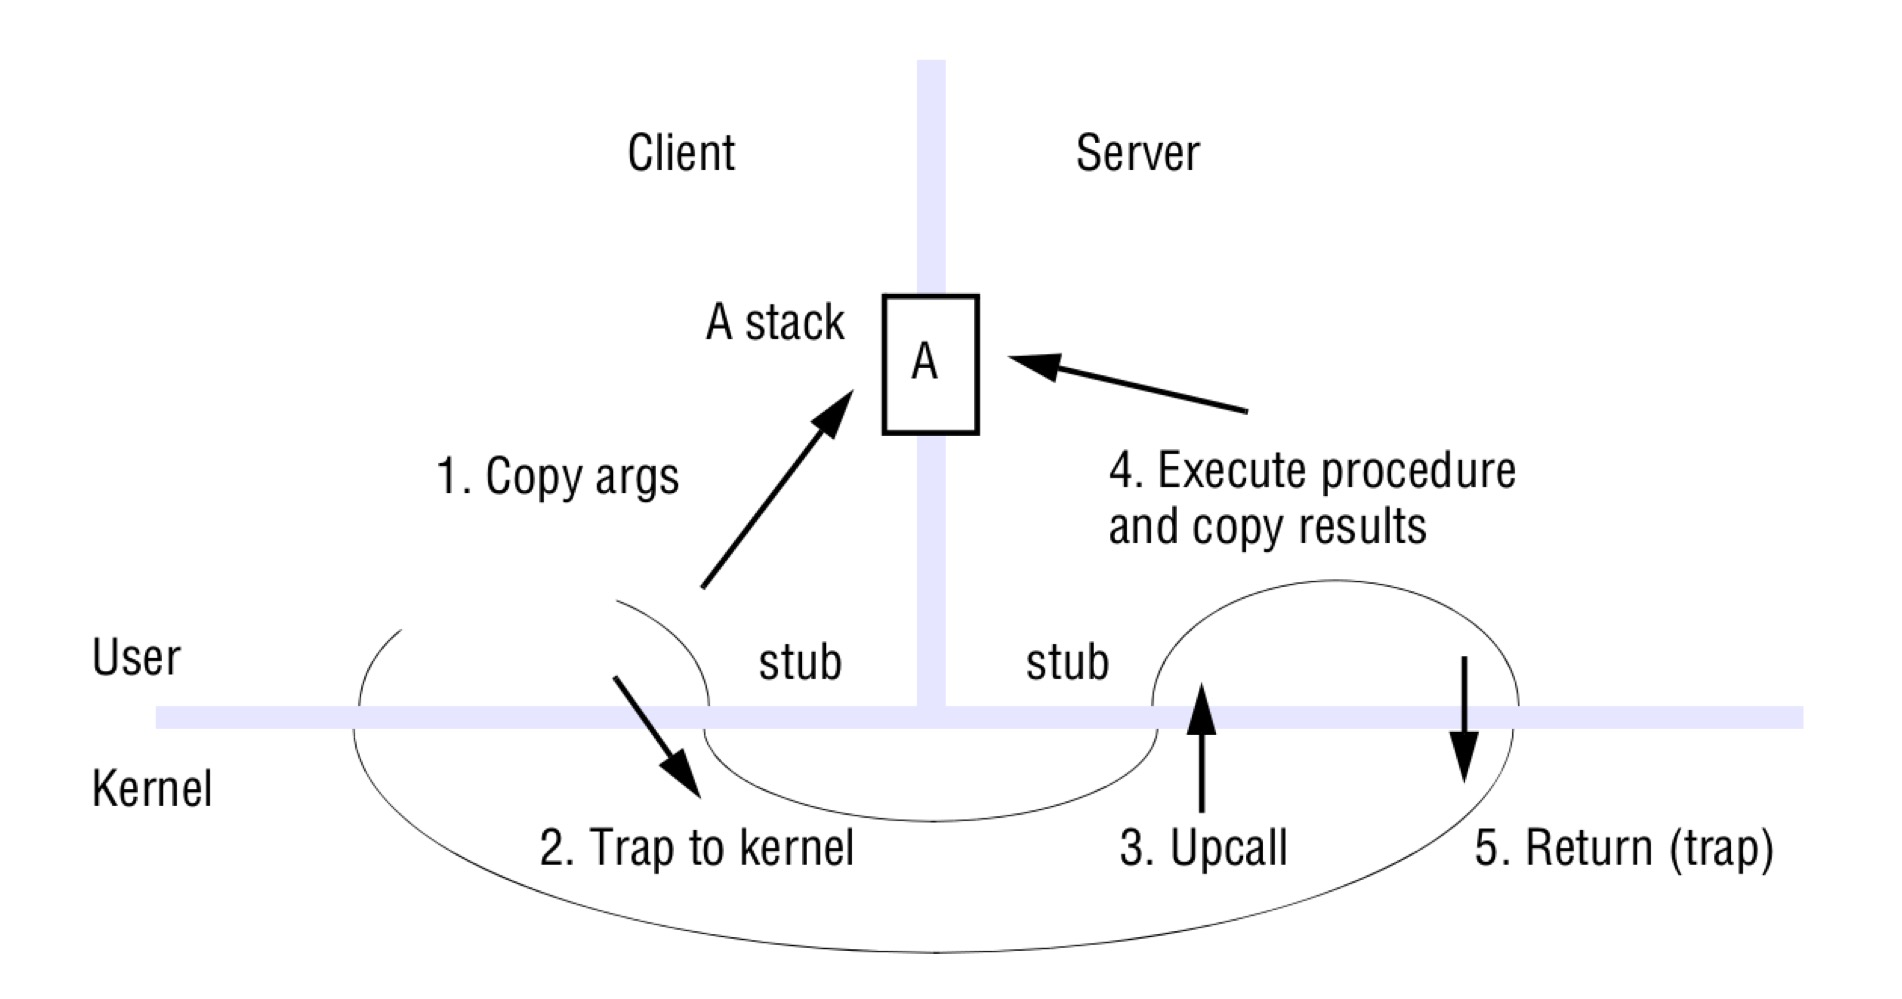
\includegraphics[width=.7\linewidth]{images/OperatingSystemSupport/LRPC.jpeg}
    \caption{LRPC}
\end{figure}

\begin{itemize}
    \item A client thread enters the server's execution environment by first tapping to the kernel and presenting it with a capability
    \item The kernel check this and only allows a context switch to a valid server procedure
    \item If it is valid, the kernel switches the thread's context to call the procedure in the server's execution environment.
    \item When the procedure in the server returns, the thread returns to the kernel, which switches the thread back to the client execution environment.
\end{itemize}

\subsection{Asynchronous operations: serialized and concurrent invocation}
With remote invocation we have some delays that have a strong impact on the final performance. The main goal of asynchronous operation is to try to limit as much as possible them. A solution is performing \textbf{concurrent invocation}, respect to \textbf{serialized one.} The following picture explain who they work.

\begin{figure}[!h]
    \centering
    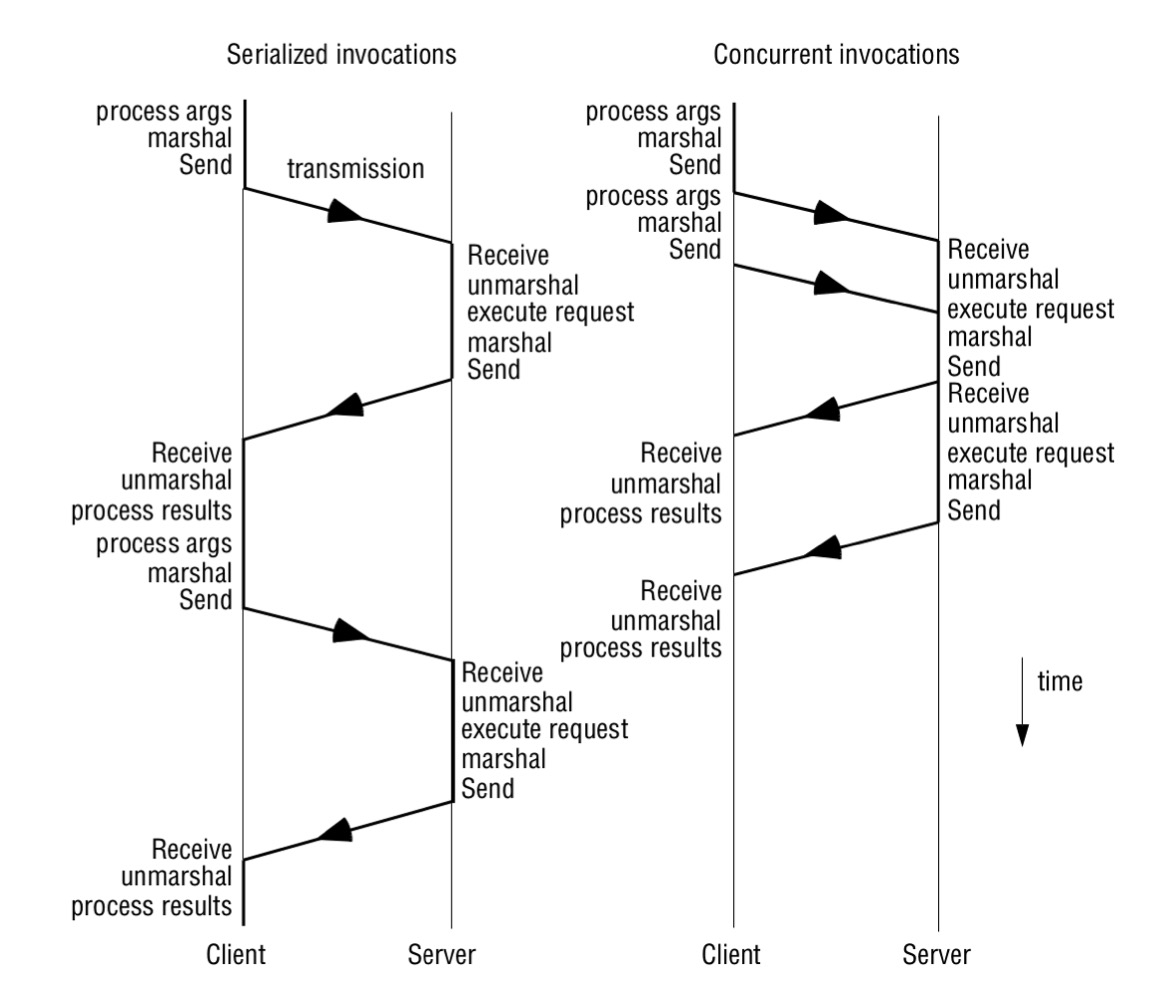
\includegraphics[width=.7\linewidth]{images/OperatingSystemSupport/serialAndCOncurrentInvocation.jpeg}
    \caption{Serial and Concurrent Invocation}
\end{figure}
\newpage
With \textbf{concurrent invocation} client allocate multiple threads to perform blocking invocations concurrently, an example is browser web.
In serialized case, the client marshal the arguments, call the \textit{Send} operation and the waits the results. After this it can make the second invocation. In the concurrent case, the first client thread marsh the arguments and calls the \textit{Send} operation. The second thread then immediately makes the second invocation. Each thread waits to receive its results.

\section{Organization and distributed operating system architecture}
Now we analyse the architecture of a kernel suitable for a distributed system. An open distributed system should make it possible to:
\begin{itemize}
    \item Run only that system software at each computer that is necessary for it to carry out its particular role in the system architecture
    \item Allow the software (and the computer) implementing any particular service to be changed independently of other facilities
    \item Allow for alternatives of the same service to be provided
    \item Introduce new services without harming the integrity of existing ones
\end{itemize}

The organization of the operating system can be:
\begin{itemize}
    \item \textbf{Monolithic}
    \item \textbf{Microkernel}
\end{itemize}
These designs differ primarily in the decision as to what functionality belongs in the kernel and what is to be left to server processes that can be dynamically loaded to run on top of it.

\subsection{Monolithic}
It perform all basic operating system functions. It is an operating system architecture where the entire set of functionalities is working in kernel space. The advantage is that it is relatively efficient.

\subsection{Microkernel}
The kernel provides only the most basic abstractions, principally address spaces, threads and local interprocess communication. Clients access these system services using the kernel’s message-based invocation mechanism. The advantages are extensibility of the system, given by its modular organization, and it is simple to debug.

\section{Scheduling: process allocation}
Allocation of processes in centralized system has the advantage of using a \textbf{unique process queue}, in some sense we have the global knowledge. So the scheduler manages that queue and applies scheduling algorithm to decide which is the next process that must be executed. \textbf{Scheduling algorithms} are designed for system performance optimization, that essentially try to minimize the response time and maximise the system resources utilization.

Under certain condition the theory provides an optimal algorithms for process schedulting. In \textbf{multiprocess system} also we have a unique process queue, but now the system is composed by multiple processors.

In distributed system process allocation is more complicated since there is not a unique process queue, processes must be allocated to different machines and migration of them can occur.

Scheduling in distributed system introduce a new target to optimize which is \textbf{load balancing}. Load balancing consist on developing a solution / strategy that move processes between machines in order to assign the same load to the different machines.

Process allocation could be classified in this way:
\begin{itemize}
    \item \textbf{Static / Dynamic} if allocation decision are prefixed or not
    \item \textbf{Deterministic / Non-deterministic} if next process requests are known
    \item \textbf{Centralized / Distributed / Hierarchical}
    \item \textbf{Optimal / Approximated}
    \item \textbf{With / Without Migration}
\end{itemize}


\section{Scheduling algorithms for distributed systems}
We can have different scheduling algorithms:
\subsection{Probes algorithm}
When the processor executing the process becomes overloaded it takes the decision to transfer the process, \textbf{probes} another processor the decide whether to transfer the process. If the contacted processor is \textbf{underloaded} the transfer takes places, otherwise it selects randomly another processor to repeat the attempt up to a maximum number of times.

\subsection{Deterministic algorithm}
Here we have \textit{n} processes to distribute on \textit{k} identical processors \((n > k)\). There is an \textbf{assumption:} the \textbf{traffic} between each process couple is known. The algorithm distributes the load to minimize the total traffic among the processors. The \textbf{drawbacks} of this strategy is the knowledge of the traffic distribution, the traffic information and deal with change of variation of it.

\subsection{Centralized algorithm}
It is centralized algorithm to \textbf{distribute the load} between workstations for load balancing. Each workstation has a \textbf{score} and if it sends information to other process the score increase, if it serves others the score decreases.

\subsection{Bidding algorithm}
It is an extension of centralized algorithm. It is based on the \textbf{metaphor of an economic system}, where CPU time is associated to a price. Each processor computes the \textbf{offered price} according to the demands and quality of service. The algorithm evaluates the most convenient choice for each process to be executed. 

\subsection{Hierarchical algorithm}
The hierarchical algorithm \textbf{improves the scalability} of the scheduler. Processes are organized based on an \textbf{hierarchical organization} in which each \(K\) processors has a \textbf{supervisor} that keeps the information about the single \(K\) workload and the number of available processors. We can have different levels of organization, and it is more fault tolerance since in case of crash of the supervisor \textbf{substitution mechanisms} are used to substitute it.

\subsection{Coscheduling}
An algorithm can consider the communication among processes to allocate strongly connected processes on the same node. It is convenient to keep together communicating processes, in order to reduce communication delays. A common representation used for this algorithm is based on the \textbf{usage of a matrix} in which \textit{rows} represent time units and \textit{columns} represent processors. The location \textit{(i, j)} contains the id of the process to be executed at time \textit{i} on processor \textit{j}. 
